% DA RISCRIVERE DISTRIBUENDO IL CONTENUTO NEI VARI ALTRI BULLET POINTS DI QUESTA SEZIONE
% Our scenario has a swarm in which one of the drones acts as an anchor.
% The anchor is allowed to move independently and faster, while keep moving in the same direction of the swarm.
% The objective is to move collect the measurement in four points relatively to the reference frame in which we consider the swarm, to collect the data required by the algorithm (WLP and MDS)
% The algorithms have been tested in two type of simulated environments: 
% The first with a node simulating the dynamic of the drones, capable of managing more than 10 drones and which allows us to perform our studies.
% The second with Gazebo+Ardupilot, for performing a simulation with the SITL and getting closer to a real application of the algorithm on physical robots. Unfortunately, this version is computational-heavy and we were able to run the simulation with XX drones at the most.
% In both cases, the operating entities were executing in a ROS 2 project object of our work.
% Sottolineare che abbiamo la simulazione con test e la simulazione con Gazebo. ABbiamo fatto test perchè più veloce.
% Activity diagram per spiegare i passaggi, quasi impostato come macchina a stati finiti.
% Dire che abbiamo usato ROS 2, foto dei topic sia stilizzata che completa in appendice con 10 droni
% Foto Gazebo con il mondo con i dron


\section{Methodology}\label{sec:methodology_section}
This section describes the main aspects of the implementation not yet adequately depicted and the methodologies employed to verify the performances of the discussed techniques.
The implementation consists of a ROS 2 project where the goal is to estimate the position of the drones in a swarm using the measurements of their relative distances. The swarm operates in a simulated environment, which can be of two types. In the first type, a dedicated ROS 2 node is responsible for simulating the drones dynamics solely via numerical integration, while the second adopts the physical simulator Gazebo\footnote{https://gazebosim.org/home}. 
To make this second simulation even more realistic, the commands are routed through ArduCopter\footnote{https://ardupilot.org/copter/} via Mavros\footnote{https://github.com/mavlink/mavros}.

The reason why two simulation types were developed is twofold. First, in this way the project is more modular and scalable. Second, running a simulation with Gazebo and a Mavros node for each drone is computational heavy and no adequate computational resources were available for this purpose. Still, the Gazebo+Ardupilot combination serves the purpose of closely simulating the Software-In-The-Loop (SITL) environment, bridging the gap towards real-world deployment.
Figure~\ref{fig:gazebo_setup} illustrates the Gazebo setup in the case of 3 drones.

\begin{figure}[!ht]
  \begin{center}    
    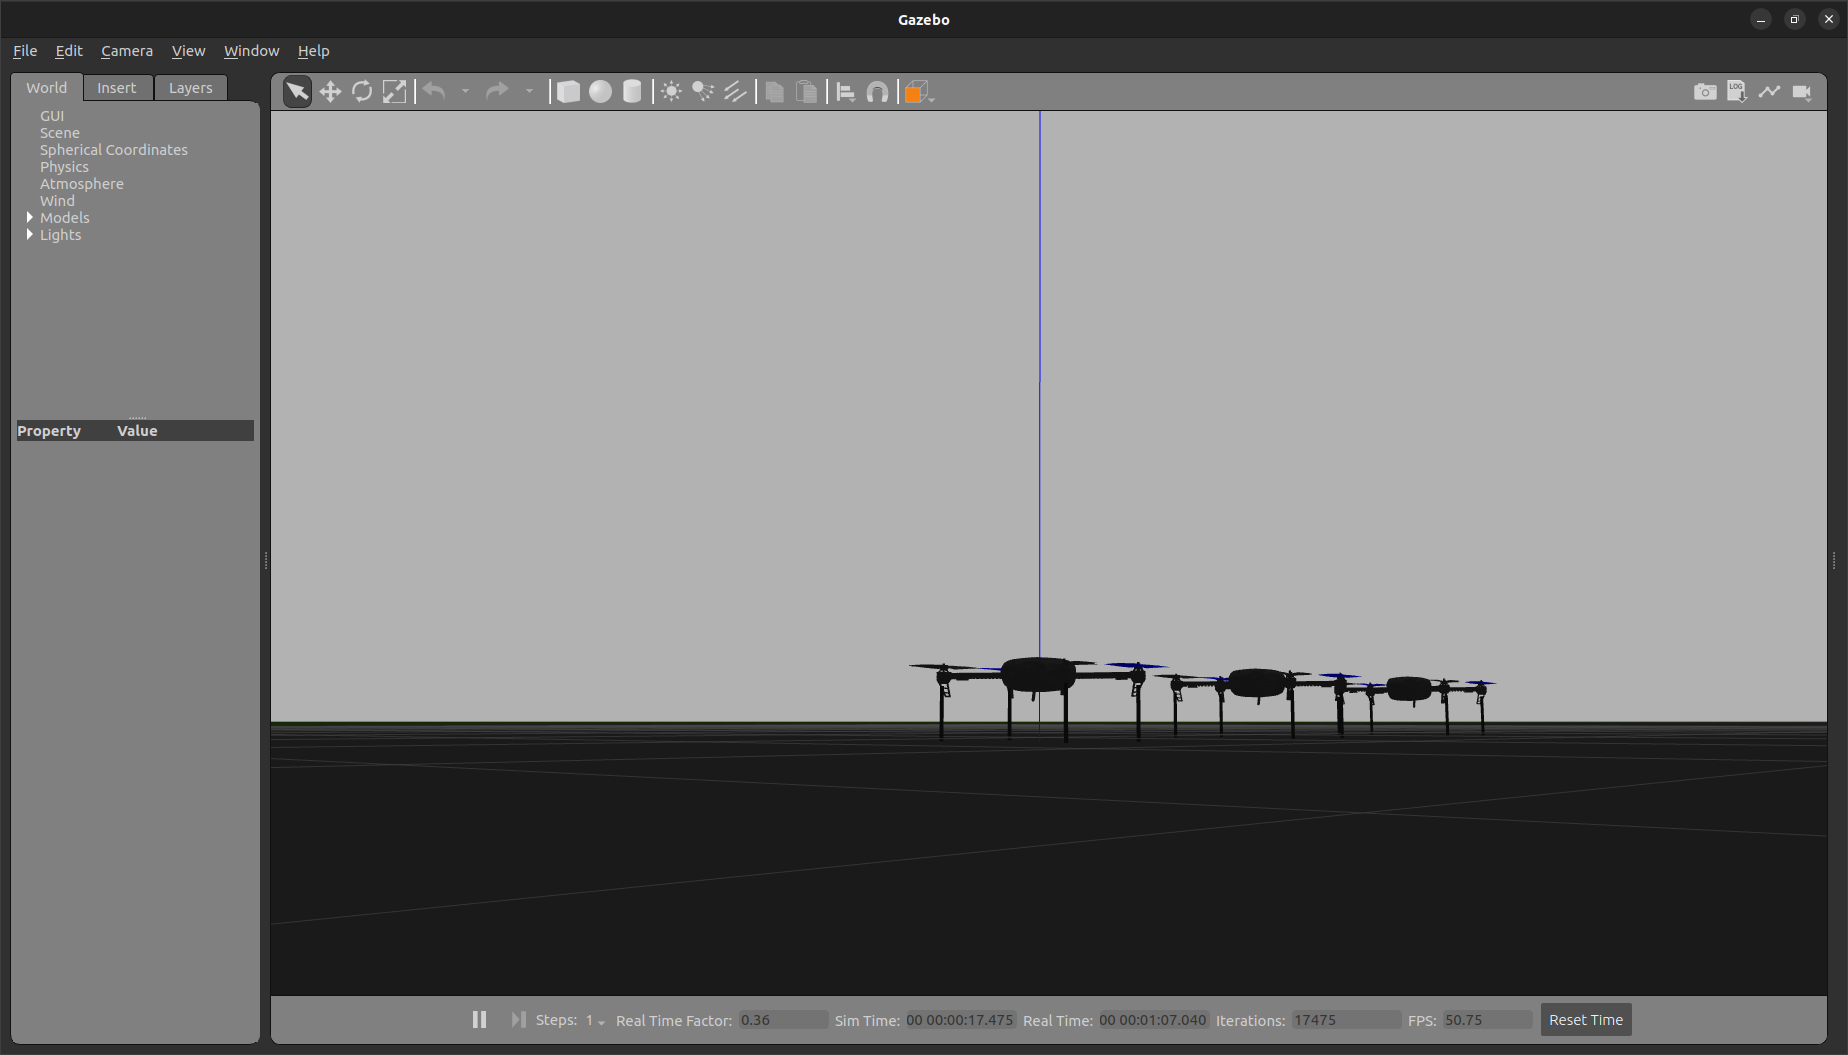
\includegraphics[width=0.45\textwidth]{figures/gazebo-environment.png}
  \end{center}
  \caption[Gazebo setup]{
    \textbf{Gazebo setup.} 
    Gazebo simulator and runway world for simulating the guidance of a swarm of drones while estimating their positions.
  }
  \label{fig:gazebo_setup}
\end{figure}

In the following, the process regarding the data collection for such scenario will be better explained. Subsequently, the blocks composing the ROS 2 project will be better illustrated, highlighting how they interact, both in the case of simple numerical simulator and with Gazebo. Finally, the experiment procedure will be exposed and explained, leading to the comparison of the two algorithms, i.e. trilateration and MDS.



\subsection{Infrastructure-free localization}
In this section, the approach for an infrastructure-free localization of drones is presented, operating within a WSN. 
Unlike traditional methods that rely on a fixed set of anchor nodes to determine drone locations, this research embraces a novel approach inspired by recent trends in the literature. This approach involves designating a single drone within the swarm as the “anchor node”, which moves faster than the others and is in charge of collecting distance measurements from various points.
As reiterated multiple times, both of the compared algorithms are only able to solve the problem if equipped with 4 sets of measurements from distinct points. 

In the project, the reference system with respect to which the positions of the drones are calculated is centered at the position of the anchor. In both the simulation types, the drone designated as the anchor is the one called \textit{drone1}. In the case of the numerical simulation, its initial position is $x_0^1=[0.0,0.0,5.0]^\top$\footnote{In the notation, subscript refers to time, and superscript to drone.}, while in Gazebo it is in at the origin of the absolute reference frame. 
In contrast, the position of the other drones is randomly generated in all coordinates. \par

During the simulation, the swarm is moved at a constant speed in a predefined direction. 
The anchor drone is subject to the same movement of the swarm, but, in addition to it, it also continuously changes its position to collect new measurements from different points.
This is achieved by imposing to the anchor not only the swarm velocity, but also an additional one depending on the direction it has to follow. \par

Once the anchor has moved in a certain direction for a given time (which can be affected by noise), it remains still relatively to the swarm, to complete the distances collection and perform an estimation of the swarm configuration through the localization algorithms.
After this, a new direction is assigned to the anchor and the cycle is repeated. Figure~\ref{fig:flowchart} presents a flowchart with the main steps of the described approach, while Figure~\ref{fig:sequence} the screenshots obtained by executing the project with no noise for an anchor movement.

\begin{figure}[!ht]
  \begin{center}
    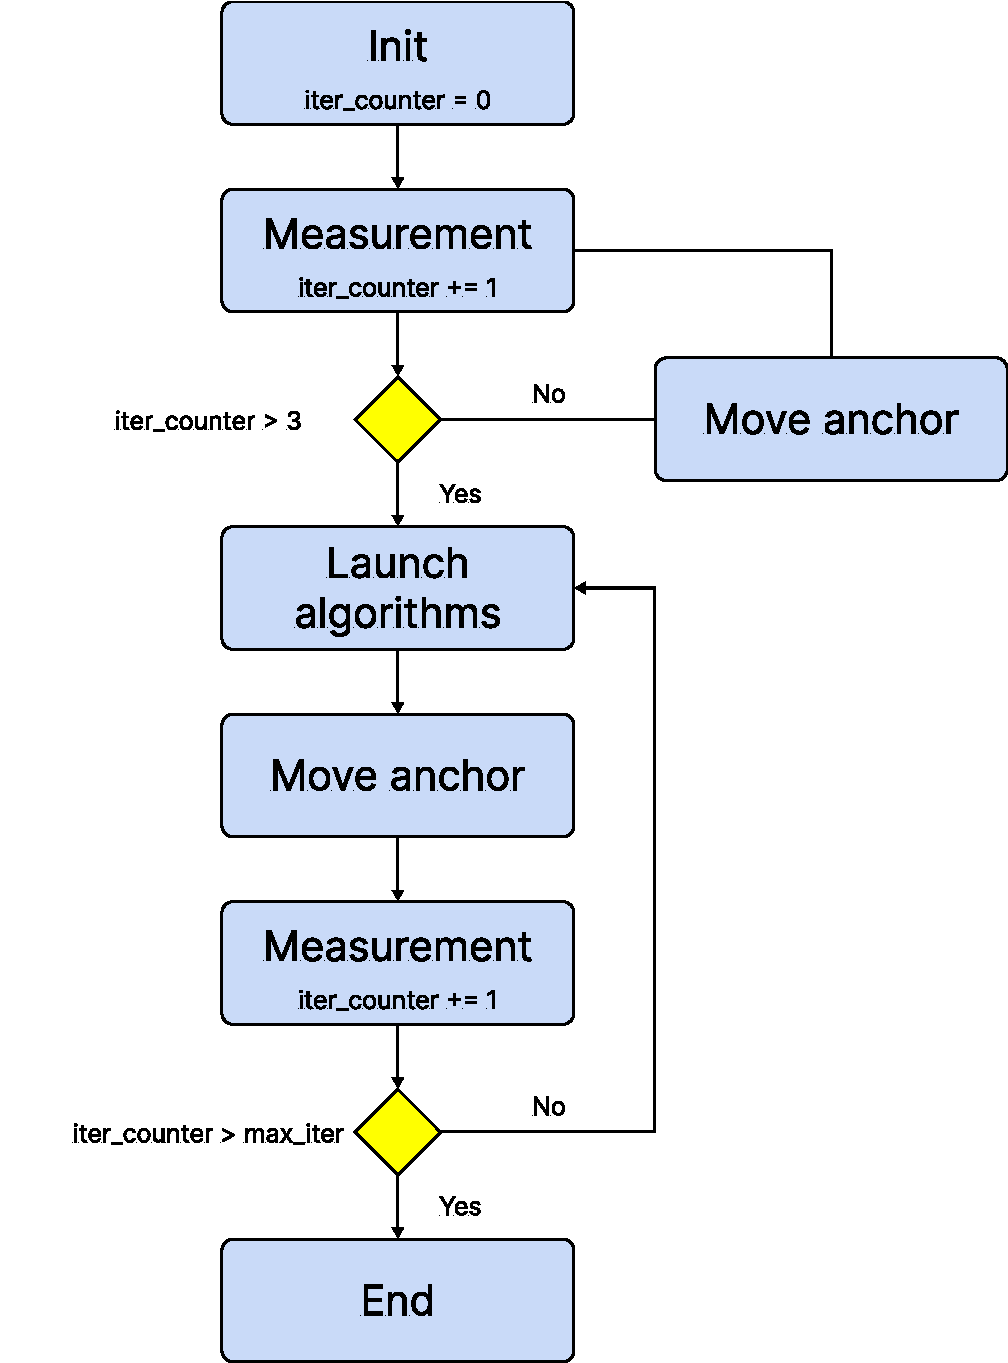
\includegraphics[width=0.37\textwidth]{figures/flowchart_color.pdf}
  \end{center}
  \caption[Software flowchart]{
    \textbf{Software flowchart.} 
    The diagram illustrates the main steps of the implemented approach. This was used for both the simulation types. The first loop is necessary to make sure to have at least four sets of measurements. The second cycle, on the other hand, is the one continuously performed to estimate the drones position.
  }
  \label{fig:flowchart}
\end{figure}


\begin{figure*}[!ht]
     \centering
     \begin{subfigure}[b]{0.28\textwidth}
         \centering
         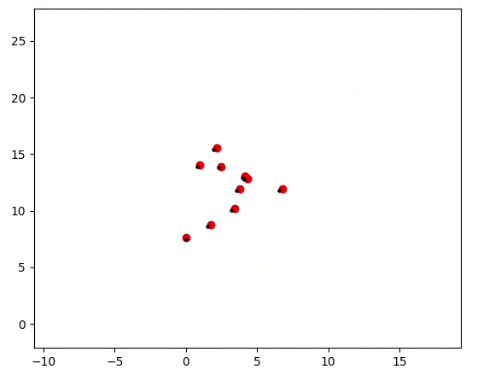
\includegraphics[width=\textwidth]{figures/sequence_1.png}
         \caption{Step 1.}
         \label{fig:sequence_1}
     \end{subfigure}
     \hfill
     \begin{subfigure}[b]{0.28\textwidth}
         \centering
         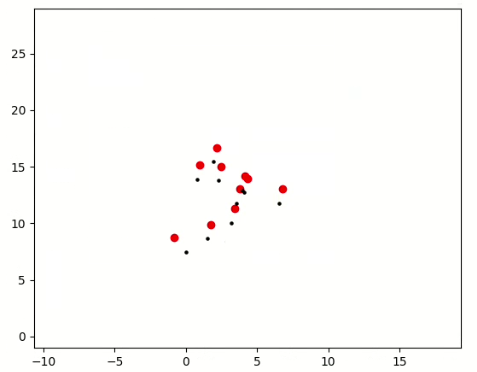
\includegraphics[width=\textwidth]{figures/sequence_2.png}
         \caption{Step 2.}
         \label{fig:sequence_2}
     \end{subfigure}
     \hfill%
      \begin{subfigure}[b]{0.28\textwidth}
         \centering
         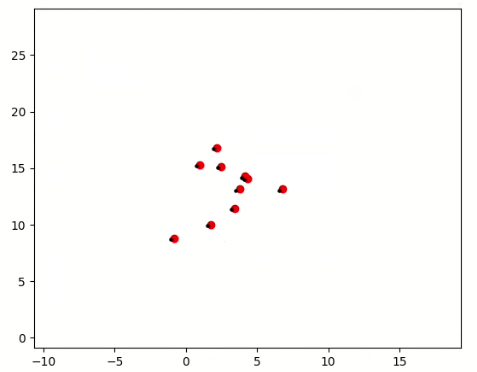
\includegraphics[width=\textwidth]{figures/sequence_3.png}
         \caption{Step 3.}
         \label{fig:sequence_3}
     \end{subfigure}
     \hfill
     \caption[Algorithm iteration]{
        \textbf{Algorithm iteration.} 
        This screenshots illustrate the main steps of an iteration of the algorithm. The anchor starts moving from a point in which the data collection and estimation have been performed (\ref{fig:sequence_1}). While moving, the rest of the swarm moves toward a predefined direction, positive $y$ in the case shown (\ref{fig:sequence_2}). After a given time, the anchor stops and remains in the same relative position for a new data collection and estimation, until the next iteration (\ref{fig:sequence_3}). 
      }
     \label{fig:sequence}
\end{figure*}


\subsection{Architecture}
The project is built upon ROS 2, with key nodes designed to fulfill specific roles within the system architecture.
The core node is the one called \textit{main}, which is responsible for guiding drones, reading distance measurements, running algorithms and tracking results. 
Another important node, called \textit{hub}, reads the coordinates from the environment (either the numerical simulator or Gazebo) and returns the distances, possibly adding noise. This functionality simulates the adoption of real UWB sensors. 

The numerical simulator node (i.e. \textit{test}) is responsible for tracking drones' positions, simulating the application of velocity commands, and incorporating dynamic model noise to represent real-world motion behaviors.
Other nodes were adopted when using Gazebo: the Mavros nodes, for communicating between the scripts, and the Ardupilot plugin.

The simplified diagram in Figure~\ref{fig:nodes_architecture} provides a visual representation of the simulation setup, highlighting the main nodes and topics\footnote{In ROS 2, a topic is a named channel of communication that facilitates the exchange of data between different nodes.}. 
The diagram resembles the one obtained by launching the rqt\_graph\footnote{http://wiki.ros.org/rqt\_graph} tool. For clarity, only the connections of 3 drones are illustrated.

% The diagram resembles the one obtained launching the rqt\_graph \footnote{http://wiki.ros.org/rqt_graph} tool, but, for clarity, only 3 drones are considered in the diagram, but when using the numerical simulator more nodes can be managed. On the other hand, when using Gazebo, we were able to run the simulation with three drones at the most. % Appendix A provides the diagram obtained running the rqt\_graph\footnote{http://wiki.ros.org/rqt_graph} tool when Gazebo is operating.

\begin{figure}[!ht]
  \begin{center}
    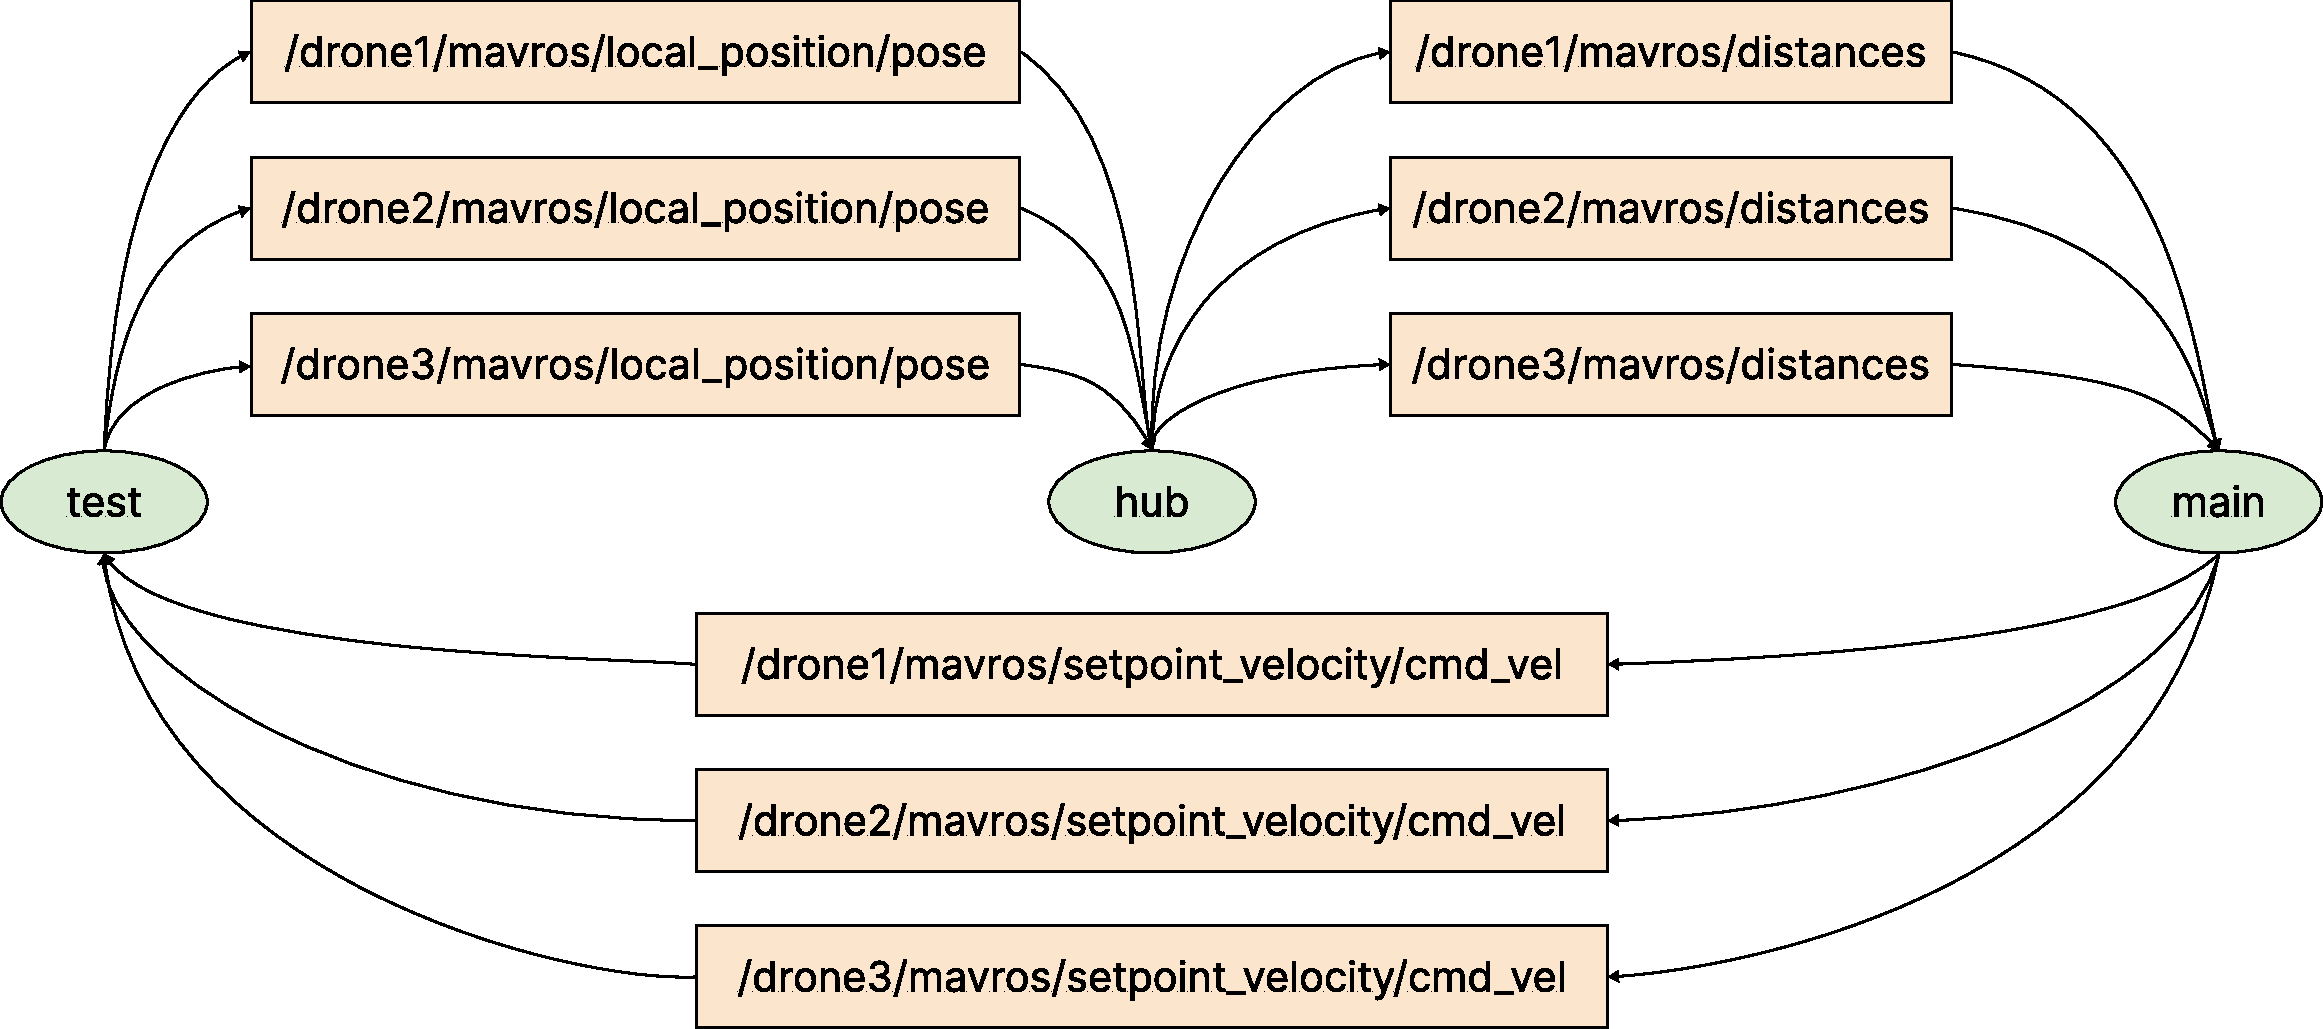
\includegraphics[width=0.47\textwidth]{figures/nodes_architecture_color.pdf}
  \end{center}
  \caption[Nodes architecture]{
    \textbf{Nodes architecture.} 
    Graph showing the connections between the main nodes operating when running the project for 3 drones with the numerical simulator. Each node is represented with an ellipse, while the topics are in rectangles. The graph has bee redrawn from that obtained using the rqt\_graph tool. Some of the connections needed in the real implementation have been deleted for clarity.
  }
  \label{fig:nodes_architecture}
\end{figure}

\subsection{Experimental setup}
To evaluate the performance of the two algorithms, a series of targeted experiments was carried out, mostly using the numerical simulator. 
This approach enabled to run multiple experiments with different settings and aggregate performance metrics for robust conclusions. 
These experiments encompassed distinct settings, each characterized by specific noises. The types of noise considered are: $a)$ the noise affecting the distance measurement, which is set by the hub; $b)$ the noise that affects the time for which a node continues to move along a specific direction, compromising the accurate knowledge of the anchor position; $c)$ a noise affecting the system dynamics.\par

All the noises are assumed to come from Gaussian distributions centered in zero and with a standard deviation specified via parameters.\par

The algorithms were assessed across five distinct settings: no noise, one noise out of three per time, and all three present together. Table~\ref{tab:std_summary_comparison} summarizes the standard deviations characterizing the different noises for the tested setting. 
\begin{table}[!ht]
    \centering
    \begin{tabular}{l|ccccc}
      \textbf{Quantity} & 
      \textbf{setting1} &
      \textbf{setting2} &
      \textbf{setting3} &
      \textbf{setting4} & 
      \textbf{setting5} \\
      \hline
      Distance [m]& 0.0 & 0.05 & 0.0   & 0.0 & 0.05   \\
      Time [s] & 0.0 & 0.0  & 0.0   & 0.2 & 0.2    \\
      Dynamics [m]& 0.0 & 0.0  & 0.001 & 0.0 & 0.001  \\
    \end{tabular}
      \caption[Setting details]{
        \textbf{Setting details.}
        The standard deviations of the Gaussian-distributed, zero-mean noises affecting the considered quantities is reported for the different tested settings.
    }
    \label{tab:std_summary_comparison}
\end{table}


Each setting underwent 50 runs with 33 anchor movements and 30 algorithm executions (i.e. 30 iterations of the second cycle in the diagram in Figure~\ref{fig:flowchart} started after having collected 3 set of measurement). Each time the project is executed, the number of drones can be specified by a parameter. For data collection, the control of 10 drones was simulated, whose location is randomly generated using the number of runs being tested as a seed\footnote{In the context of a random number generator (RNG), a seed is an initial value that is used to start the generation process. It serves as the starting point for producing a sequence of seemingly random numbers.}, so that the comparison between different settings is fair. In addition, to facilitate the comparison and make it more meaningful, average errors are calculated by grouping both by setting and drone, as shown in the following section.
